\documentclass{report}
\usepackage{subcaption}
\usepackage{graphicx}
\usepackage[spanish,es-tabla]{babel}
\usepackage[spanish]{babel}
\usepackage[utf8]{inputenc}
\bibliography{referencias}

\begin{document}
	\begin{titlepage}
		\centering
		{\bfseries\LARGE Universidad Privada de Tacna \par}
		\vspace{1cm}
		{\scshape\LARGE Facultad de Ingenier\'ia de Sistemas \par}
		\vspace{3cm}
		{\scshape\Huge Informe de Laboratorio N.01 \par}
		\vspace{2cm}
		{\itshape\Large SONARQUBE  \par}
		\vfill
		{\Large Autor: \par}
		{\Large Victor Piero Limache Victorio \par}
		\vfill
		{\Large 31 de Noviembre del 2020 \par}
	\end{titlepage}


	\tableofcontents
	\chapter{Introducción}
	
Sonarqube es una plataforma de codigo abierto (Software Libre) para la verificacion y mantenimiento de la calidad de codigo. Esta herramienta nos provee la covertura de los 7 pilares dentro de la calidad del codigo:Arquitectura y Disenio ,Comentarios, Reglas de Codigo,Errores potenciales ,Complejidad, Tests de Unidady Duplicaciones
\\


	\chapter{Fundamentos teóricos}
	
	\section{Teoría clásica}
	
	\subsection{Definiciones}
	
		\begin{itemize}
			\item ¿Qué es SonarQube?
			
			Profundizando un poco más lo anteriormente comentado SonarQube es una plataforma de código abierto para el análisis de la calidad de código usando diversas herramientas de análisis estático de código fuente como Checkstyle, PMD o FindBugs para obtener métricas que pueden ayudar a mejorar la calidad del código de un programa. También pertenece al conjunto de herramientas de análisis de código estático, junto con Understand, semmle y otras.\\
			
			Es una herramienta esencial para nuestra fase de testing y auditoria de código dentro de nuestro ciclo de desarrollo de nuestra aplicación. Existen muchos problemas que se pueden encontrar en un código. Las reglas difieren y pueden clasificarse en 5 grupos según su severidad: Bloqueador, crítico, grave, menor e informativo. Así que, si hay un bug o un bug potencial, va a ser clasificado como problema bloqueador o crítico, y algunos problemas como “los números mágicos no se deben utilizar” van a ser clasificados con severidad menor o informativa. Y deberá volver a la fase de desarrollo para corregir esas partes de código.\\
			
			\item ¿Por qué elegir SonarQube?
			
			No solo porque es open source si no también por la cantidad de reglas que usuarios de la comunidad que le rodea van actualizando constantemente. En este momento, existen más de 406 reglas de Java, y esta cantidad aumenta constantemente. Pueden realizarse fácilmente en códigos escritos en cualquiera de los otros 20 lenguajes de programación. Por ejemplo Python dispone de 238 reglas.\\
			

			\begin{figure}[htb]
				\centering
				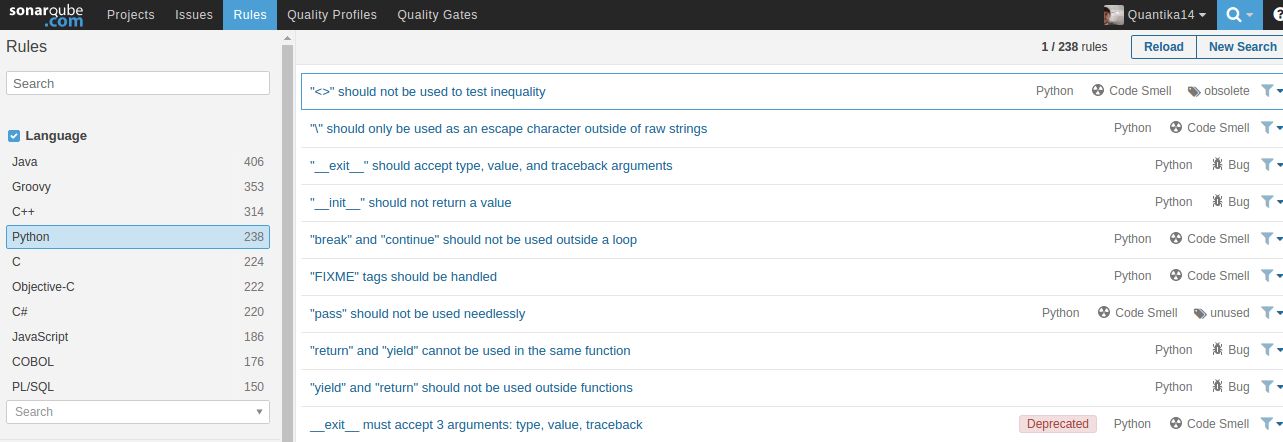
\includegraphics[width=1\textwidth]{img/ejemplo01.png}
				\label{fig:ejemplo}
			\end{figure}
			
			
		\end{itemize}
		
		
	
	
	
	\chapter{Desarrollo}
	
	\begin{enumerate}
		\item {\large Descargar SonarQube.}\\\\
		docker pull sonarqube \\ 
		
		\begin{figure}[htb]
			\centering
			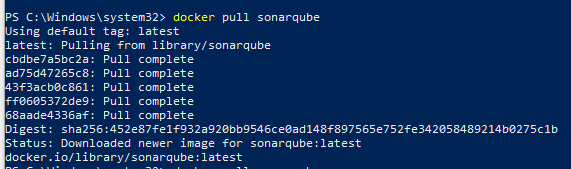
\includegraphics[width=0.8\textwidth]{img/instalacion.png}
			\label{fig:instalacion}
		\end{figure}
		
		\item {\large Ejecutar una instancia de SonarQube.}\\\\
		
		docker run -d --name sonarqube -p 9000:9000 sonarqube.\\ 
		
		\begin{figure}[htb]
			\centering
			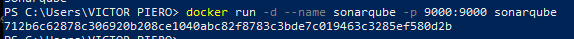
\includegraphics[width=0.8\textwidth]{img/ejecucion.png}
			\label{fig:ejecucion}
		\end{figure}
	
		\textit{Nota:Para eliminar una instancia previa puede utilizar el comando:}\\ 
		
		 docker rm -f sonarqube \\
		 
		 \begin{figure}[htb]
		 	\centering
		 	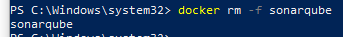
\includegraphics[width=0.8\textwidth]{img/eliminacion.png}
		 	\label{fig:eliminacion}
		 \end{figure}
		  
		\item {\large Ingresar al portal con las credenciales.}\\\\
		http://localhost:9000/ \\
		
		\textbf{user: admin}\\
		\textbf{pass: admin}\\
		
		\begin{figure}[htb]
			\centering
			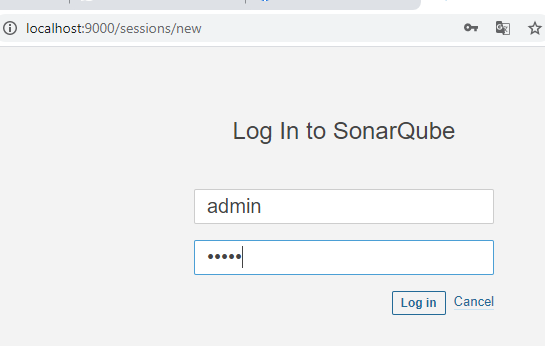
\includegraphics[width=0.8\textwidth]{img/login.png}
			\label{fig:login}
		\end{figure}
		
		
		\item {\large Crear una nueva aplicación con el nombre aplicacionNetCore.}\\\\
		
		\begin{figure}[htb]
			\centering
			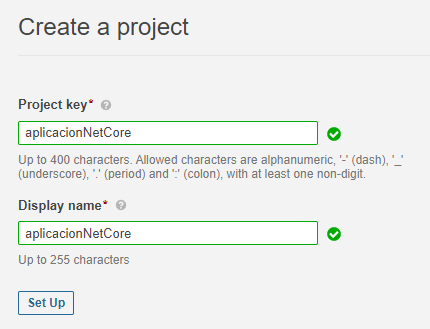
\includegraphics[width=0.8\textwidth]{img/crearproyecto.png}
			\label{fig:crearproyecto}
		\end{figure}
		
		
		
		\item {\large Generar el token de la nueva aplicación aplicacionNetCore.}\\\\
		
		\begin{figure}[htb]
			\centering
			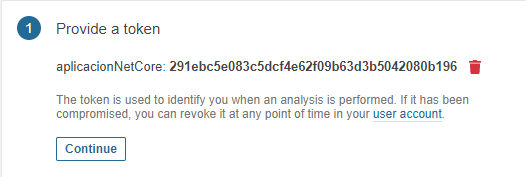
\includegraphics[width=0.8\textwidth]{img/token.png}
			\label{fig:token}
		\end{figure}
		
		\item {\large Decargar Net Core e instalar.}\\\\
		
		https://dotnet.microsoft.com/download/dotnet-core/thank-you/sdk-3.1.300-windows-x64-installer \\
		\begin{figure}[htb]
			\centering
			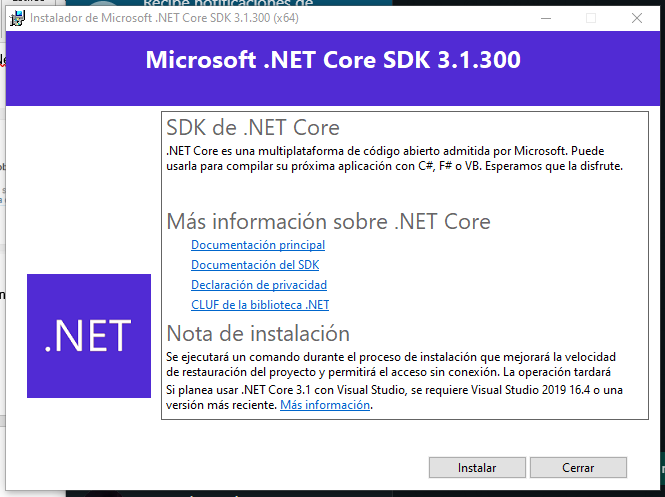
\includegraphics[width=0.8\textwidth]{img/netcoredown.png}
			\label{fig:netcoredown}
		\end{figure}
	

	
		\item {\large En un terminal ejecutar e instalar sonar-scanner.}\\\\
		
		dotnet tool install --global dotnet-sonarscanner \\
		
		\begin{figure}[htb]
			\centering
			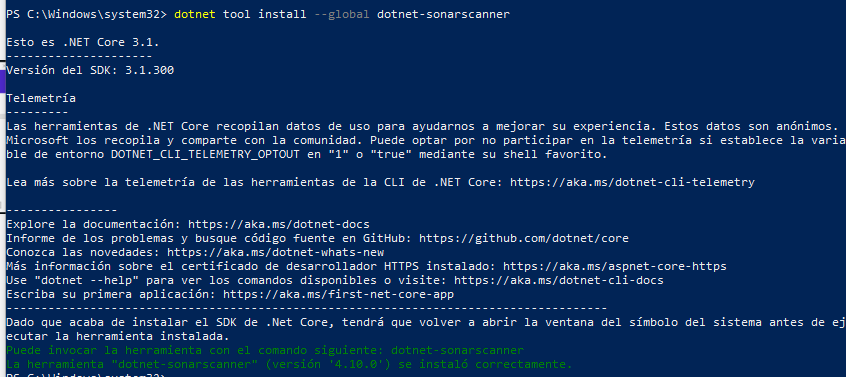
\includegraphics[width=0.8\textwidth]{img/sonarscanner.png}
			\label{fig:sonarscanner}
		\end{figure}
	
	
		\item {\large En un terminal, acceder a una ruta donde creara una nueva aplicación.} \\
		
		dotnet new sln-o aplicacionNetCore.\\
		
		cd aplicacionNetCore.\\
		\begin{figure}[htb]
			\centering
			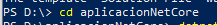
\includegraphics[width=0.7\textwidth]{img/cdaplicacion.png}
			\label{fig:cdaplicacion}
		\end{figure}
	
		dotnet new console.\\
		\begin{figure}[htb]
			\centering
			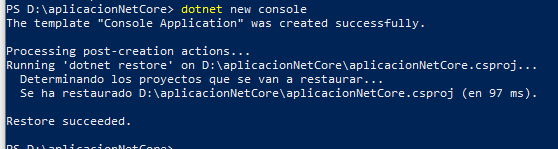
\includegraphics[width=0.7\textwidth]{img/console.png}
			\label{fig:console}
		\end{figure}
		
		dotnet sln aplicacionNetCore.sln add aplicacionNetCore.csproj \\
		\begin{figure}[htb]
			\centering
			\includegraphics[width=0.7\textwidth]{img/slnpiero.png}
			\label{fig:slnpiero}
		\end{figure}
		
		\item {\large En el mismo terminal, iniciar la sesión de revisión de sonarqube.} \\
		
		dotnet sonarscanner begin /d:sonar.host.url="http://localhost:9000" /d:sonar.login=admin /d:sonar.password=admin /k:”aplicacionNetCore” \\
		
		\begin{figure}[htb]
			\centering
			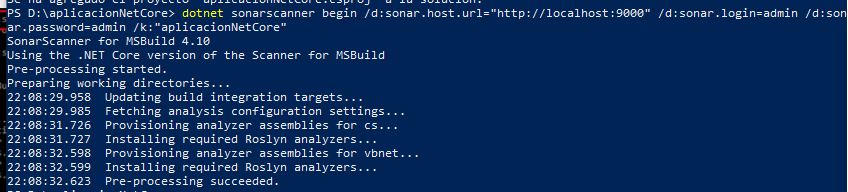
\includegraphics[width=0.7\textwidth]{img/dotnet9.png}
			\label{fig:dotnet}
		\end{figure}
		
		\item {\large Compilar la aplicación.}\\\\
		
		
		dotnet build\\
		
		\begin{figure}[htb]
			\centering
			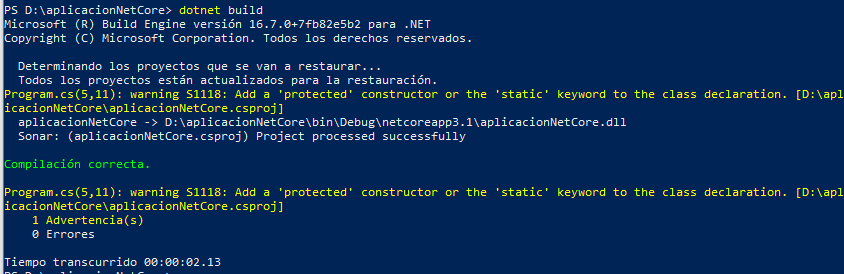
\includegraphics[width=0.7\textwidth]{img/build.png}
			\label{fig:build}
		\end{figure}
		
		\item {\large Cerramos la sesión.}\\\\
		
		dotnet sonarscanner end /d:sonar.login=admin /d:sonar.password=admin\\
		
		\begin{figure}[htb]
			\centering
			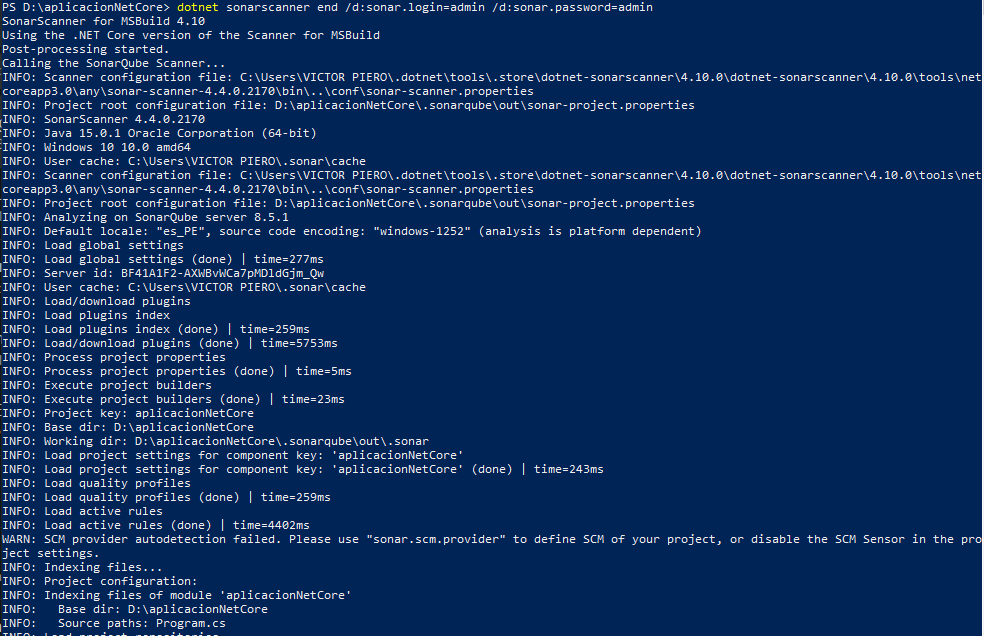
\includegraphics[width=0.7\textwidth]{img/cerrarsesion.png}
			\label{fig:cerrarsesion}
		\end{figure}
		
		\item {\large Pruebas.}\\\\
		En:  http://localhost:9000/ \\
		
		\begin{figure}[htb]
			\centering
			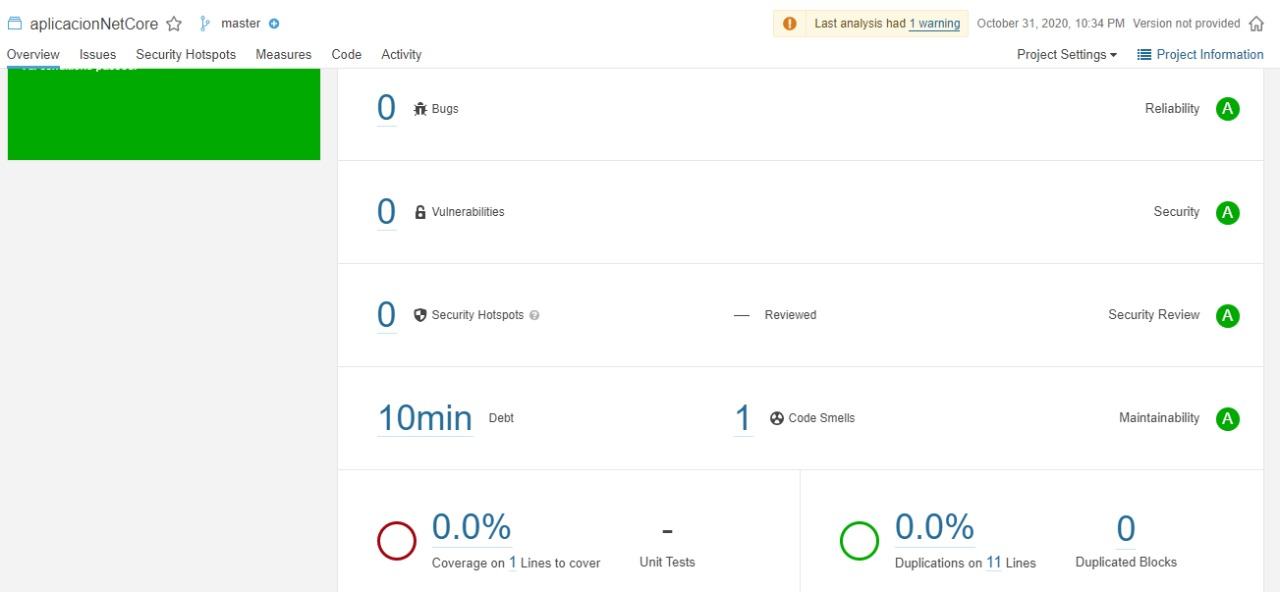
\includegraphics[width=0.7\textwidth]{img/web.png}
			\label{fig:web}
		\end{figure}
		
		En carpeta de Windows  \\
		
		\begin{figure}[htb]
			\centering
			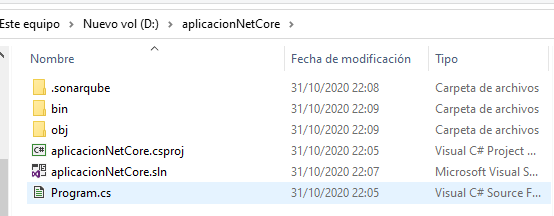
\includegraphics[width=0.7\textwidth]{img/escritorio.png}
			\label{fig:escritorio}
		\end{figure}
	\end{enumerate}
	
	\chapter{Conclusiones}
	
	Si diriges o programas algún lenguaje utilizar SonarQube es fácil de usar e instalar, ya lo veremos en la siguiente entrada, controlar la calidad de código permite disminuir la cantidad de bugs reales y potenciales. Los programadores independientemente del lenguaje que use estará más enfocado a la lógica y no invertirá tiempo en cuestiones que puede usar para encontrar soluciones óptimas para casos concretos.\\
	
	Si estás interesado en implementarlo en tu empresa puedes contactar con nosotros y si quieres saber cómo hacerlo tu mismo síguenos en las redes sociales para enterarte el primero de las siguientes entradas en el blog.\\
	
	\chapter{Bibliografia}
	
	https://blog.quantika14.com/blog/2017/05/04/que-es-sonarqube/ \printbibliography



\end{document}
